\documentclass{article}
\usepackage{graphicx} % Required for inserting images
\usepackage{amsfonts}
\usepackage{float}

\title{Note On SNARK-based ATMS}

\author{Xun Zhang \quad \quad Wuyun Siqin \quad \quad Bingsheng Zhang \\ 
Zhejiang University, CHN \\
22221024@zju.edu.cn \quad 3210101763@zju.edu.cn \quad bingsheng@zju.edu.cn}
\date{February 2025}

\begin{document}

\maketitle

\section{ATMS Construction}

We refer to the \textit{Proof-of-Stake Sidechains} paper, give both the definition and construction of ATMS(Ad-Hoc Threshold Multisignatures) as following, see section 4.1:

\vspace{0.3cm}


\textit{We introduce a new primitive, ad-hoc threshold multisignatures (ATMS), which borrow properties from
multisignatures and threshold signatures and are ad-hoc in the sense that signers need to be selected on the
fly from an existing key set. In Section 4.3 we describe how ATMS are useful for periodically updating the "anchor of trust" that the mainchain parties have w.r.t. the sidechain they are not following.}


\textit{ATMS are parametrized by a threshold $t$. On top of the usual digital signatures functionality, ATMS also provide a way to: (1) aggregate the public keys of a subset of these parties into a single aggregate public key $avk$; (2) check that a given $avk$ was created using the right sequence of individual public keys; and (3) aggregate $t' \geq t$ individual signatures from $t'$ of the parties into a single aggregate signature that can then be verified using $avk$, which is impossible if less than $t$ individual signatures are used.}

\vspace{0.3cm}


Next we give the definition and construction of ATMS, see section 4.1 and 4.3, in this report we omit definition of correctness and security:

\vspace{0.3cm}

\textit{A t-ATMS is a tuple of algorithms $\Pi = (\mathsf{PGen; Gen; Sig; Ver; AKey; ACheck; ASig; AVer})$.
Given $d$ individual signatures $\sigma_1, \ldots, \sigma_d$, created using secret keys belonging to (not
necessarily unique) public keys $vk_1, \ldots, vk_d$ can be combined into a multisignature $\sigma = \prod_{i=1}^d \sigma_i$ that can then be verified using an aggregated public key $avk = \prod_{i=1}^d vk_i$.
Assuming $S$ is a set and $\langle S \rangle$ is a a Merkle-tree commitment to the set. Where:}


\begin{itemize}
    \item $\mathsf{PGen(1^\kappa)}$ is the parameter generation algorithm that takes the security parameter $1^\kappa$ and returns system parameters $\mathcal{P}$.

    \item $\mathsf{Gen(\mathcal{P})}$ is the key-generation algorithm that takes $\mathcal{P}$ and produces a public/private key pair $(vk_i, sk_i)$ for the party invoking it.

    \item $\mathsf{Sig}(ski, m) $ is the signature algorithm as in an ordinary signature scheme: it takes a private key and a message and produces a (so-called local) signature $\sigma$.

    \item $\mathsf{Ver}(m, pk_i,\sigma)$ is the verification algorithm that takes a public key, a message and a signature and returns true or false.

    \item $\mathsf{AKey(\mathcal{VK})}$ is the key aggregation algorithm that takes a sequence of public keys $\mathcal{VK}$ and aggregates them into an aggregate public key $avk$: given a sequence of public keys $\mathcal{VK} = \{vk_i\}_{i=1}^n$, returns $avk = (\prod_{i=1}^d vk_i, \langle \mathcal{VK}\rangle)$.

    \item $\mathsf{ACheck}(\mathcal{VK},avk)$is the aggregation-checking algorithm that takes a public key sequence $\mathcal{VK}$ and an aggregate public key $avk$ and returns true or false, determining whether $\mathcal{VK}$ were used to produce $avk$: simply recomputes it to verify $avk$.

    \item $\mathsf{ASig} (m, \mathcal{VK},\langle(vk_1; \sigma_1), \ldots,(vk_d, \sigma_d)\rangle)$ is the signature-aggregation algorithm that takes a message $m$, a sequence of public keys VK and a sequence of d pairs $\langle(vk_1; \sigma_1), \ldots,(vk_d, \sigma_d)\rangle$where each $\sigma_i$ is a local
    signature on $m$ verifiable by $vk_i$ and each $vk_i$ is in a distinct position within $\mathcal{VK}$, $\mathsf{ASig}$ combines these into a multisignature $\sigma$ that can later be verified with respect to the aggregate public key $avk$ produced from $\mathcal{VK}$ (as long as $d \geq t$, see below): 

     takes the message $m$, $d$ pairs of signatures with their respective public keys $\{\sigma_i, vk_i\}_{i=1}^d$ and $n-d$ additional public keys $\{\widehat{vk_i}\}_{i=1}^{n-d}$ and produces an aggregate signature:
    \[
    \sigma = \left ( \prod_{i=1}^d \sigma_i , \{\widehat{vk_i}\}_{i=1}^{n-d}, \{\pi_{\widehat{vk_i}}\}_{i=1}^{n-d}\right )
    \]
    where $\{\pi_{\widehat{vk_i}}\}_{i=1}^{n-d}$ denotes the (unique) inclusion proof of $\{{\widehat{vk_i}}\}_{i=1}^{n-d}$ in the Merkle commitment.

    \item $\mathsf{AVer}(m,avk,\sigma)$ is the aggregate-signature verification algorithm that takes a message $m$, an aggregate publickey $avk$, and a multisignature $\sigma$, and returns true or false:
    
    \begin{enumerate}
        \item verifies that each of the public keys $\widehat{vk_i}$ indeed belongs to a different leaf
        in the commitment $\langle \mathcal{VK}\rangle$ in $avk$ using membership proofs $\pi_{\widehat{vk_i}}$.
        \item computes $avk'$ by dividing the first part of $avk$ by $\prod_{i=1}^{n-d} \widehat{vk_i}$.
        \item returns true if and only if $d \geq t$ and the first part of $\sigma$ verifies as a $\Pi_\mathsf{MGS}$-signature
        under $avk'$
    \end{enumerate}

    
\end{itemize}


\section{SNARK-based ATMS}

\subsection{Relations in Paper}
In the SNARK version of ATMS(see section 5.3 ATMS From Proofs of Knowledge) , we have a $avk$ as the root of a Merkle tree containing $\mathcal{VK}$. And let $S' = \{s_i\}$ be the signatures generated by a sequence $\mathcal{VK}'$ containing keys in $\mathcal{VK}$. The signing algorithm reconstructs the Merkle tree from
$\mathcal{VK}$ and determines the membership proof $\pi_i$ for each $vk_i \in \mathcal{VK}'$. 

The statements of SNARK is $x = (avk,m)$, and the witness of SNARK is $w = \{\pi_i, (s_i,vk_i)\}_{i \in S'}$. The SNARK system prove the following relations:
\begin{itemize}
    \item For all $i$, the signature verifying algorithm $\mathsf{Ver}(vk_i,m,s_i)$ returns true.
    \item For all $i$, proof $\pi_i$ is a valid Merkle path proof pointing to a unique leaf.
    \item $|S'| \geq t$.
\end{itemize}

This is very similar to the code implemented by Inigo, but the original code replace the Merkle tree by a straight hash.

\subsection{Code Implementation}

According to the relations mentioned in the paper, the code implementation is as following(Inigo's code, "sidechains-zk"):

\vspace{0.5cm}

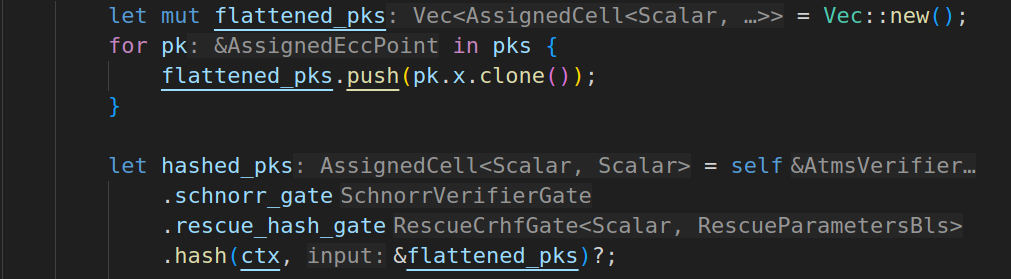
\includegraphics[width=1\linewidth]{inigo_atms_code_keyhash.png}
\vspace{0.1cm}

Compute a straight hash of all public keys firstly, and compare it to the public commitment.

Then, just as described in the paper, we verify the individual signature one by one. And if there exits a signature corresponding to a public keys, which can also be verified, we add the counter(to compute the threshold).


\vspace{0.5cm}

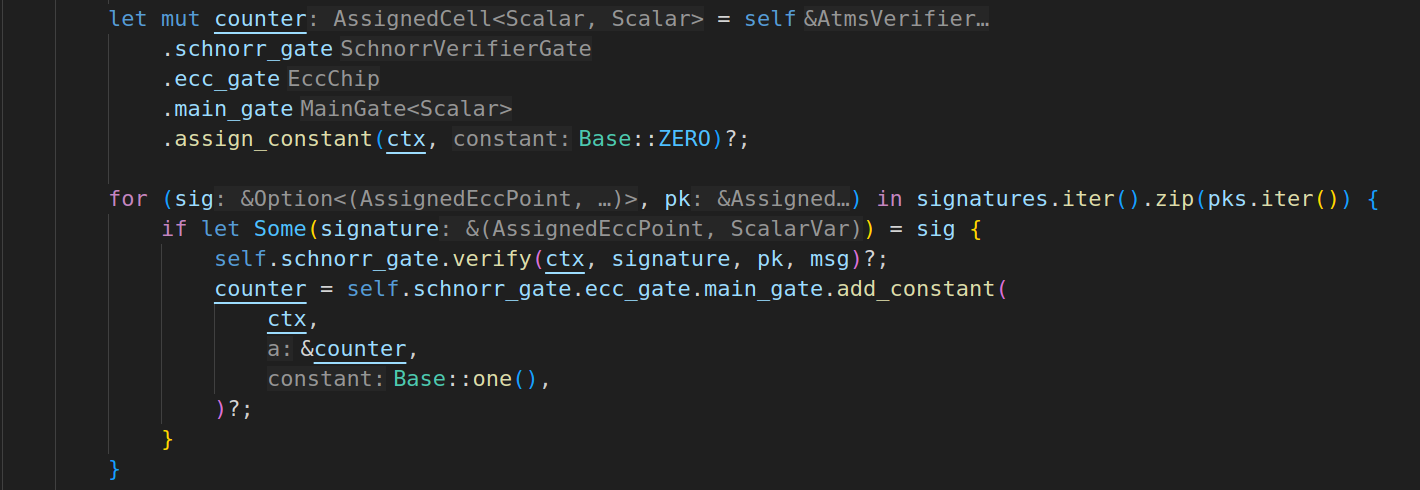
\includegraphics[width=1\linewidth]{inigo_atms_code_verify.png}
\vspace{0.1cm}


Finally we constraint the counter to be equal with threshold.

\vspace{0.5cm}

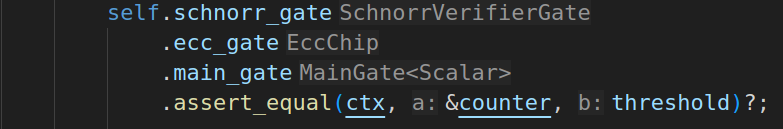
\includegraphics[width=1\linewidth]{inigo_atms_code_threshold.png}
\vspace{0.1cm}


\subsection{Our proposal}

If we use the settings in the ATMS paper, which means that there do exit a Merkle tree that commits $\mathcal{VK}$. And we need a product of all public keys $ ivk = \prod_{i=1}^n vk_i$ at first. Now, let the $avk$ be aggregated public key $avk =  \prod_{i=1}^d vk_i$, and $\sigma = \prod_{i=1}^n \sigma_i$ be the aggregated signature.

Then the statements of SNARK is $x = (avk,ivk,m,\sigma)$, and the witness of SNARK is $w = \{\{\pi_i, vk_i\}_{i \notin S'}, \{\sigma_i\}_{i \in S'}\}$. The SNARK prove the following relations:

\begin{itemize}
    \item $avk = ivk - \prod_{i=1}^{n-d} vk_i$.
    \item For all $i$, proof $\pi_i$ is a valid Merkle path proof pointing to a unique leaf.
    \item $\sigma = \prod_{i=1}^d \sigma_i$.
    \item The signature verifying algorithm $\mathsf{Ver}(avk,m,
    \sigma)$ returns true.
\end{itemize}


This is a normal multisignature-like proving approach.


\subsection{Proving Cost}

The SNARK-based ATMS implementation(Inigo's code) use Schnorr signature as its core signature scheme, but when we turn to \textbf{BLS} signature, the proving cost will increase rapidly.

Assuming the threshold is $d$, the original approach in paper need to prove(in BLS setting):

\begin{itemize}
    \item $d$ BLS signature verification.
\end{itemize}

Which means it need to prove $d$ times of pairing check, it is very costly.


In our approach, we need to prove:

\begin{itemize}
    \item Product of unused keys, signatures and the result of $avk$.
    \item $n-d$ times of Merkle path verification.
    \item $1$ BLS signature verification.
\end{itemize}


The main cost is Merkle path verification, it may can be optimized by our shuffle argument.


\subsection{Benchmark Result}

Below are SNARK benchmarks of our proposal, we use BLS signature scheme. The $num $ field indicates the number of public keys we choose to sign the message, the latter number is the total number of Merkle tree nodes.

\begin{table}[htbp]
    \centering
    \renewcommand{\arraystretch}{1.1} % 增加行间距
    \setlength{\tabcolsep}{10pt}      % 增加列间距
    \begin{tabular}{c|c|c|c} \hline
        \textbf{num} & \textbf{proof\_time} & \textbf{proof\_size} & \textbf{verify\_time} \\ \hline
        16 of 32    & 29.24s  & 13152  & 15.07ms  \\
        32 of 64    & 30.75s  & 14528  & 12.93ms  \\
        64 of 128   & 36.50s  & 17984  & 16.33ms  \\
        128 of 256  & 51.53s  & 25600  & 16.60ms  \\
        256 of 512  & 82.75s  & 41856  & 23.04ms  \\
        512 of 1024 & 147.84s & 76672  & 35.33ms  \\
        1024 of 2048 & 289.60s & 151488 & 56.85ms  \\ \hline
    \end{tabular}
    \label{tab:example_benchmark_selected}
\end{table}

Currently, the main bottleneck lies in the hash verification process used for Merkle tree validation. However, we need to adjust our parameters. Under the actual ATMS configuration, about two-thirds of the keys would be used for signing. Because the Merkle paths to be verified correspond to keys that are not signed, the real-world verification time will be lower than the current test results. 
\newpage

The figure below shows that, under the current parameter settings, both the proving time and the verification time increase linearly with the number of keys.
\begin{figure}[htbp]
    \centering
    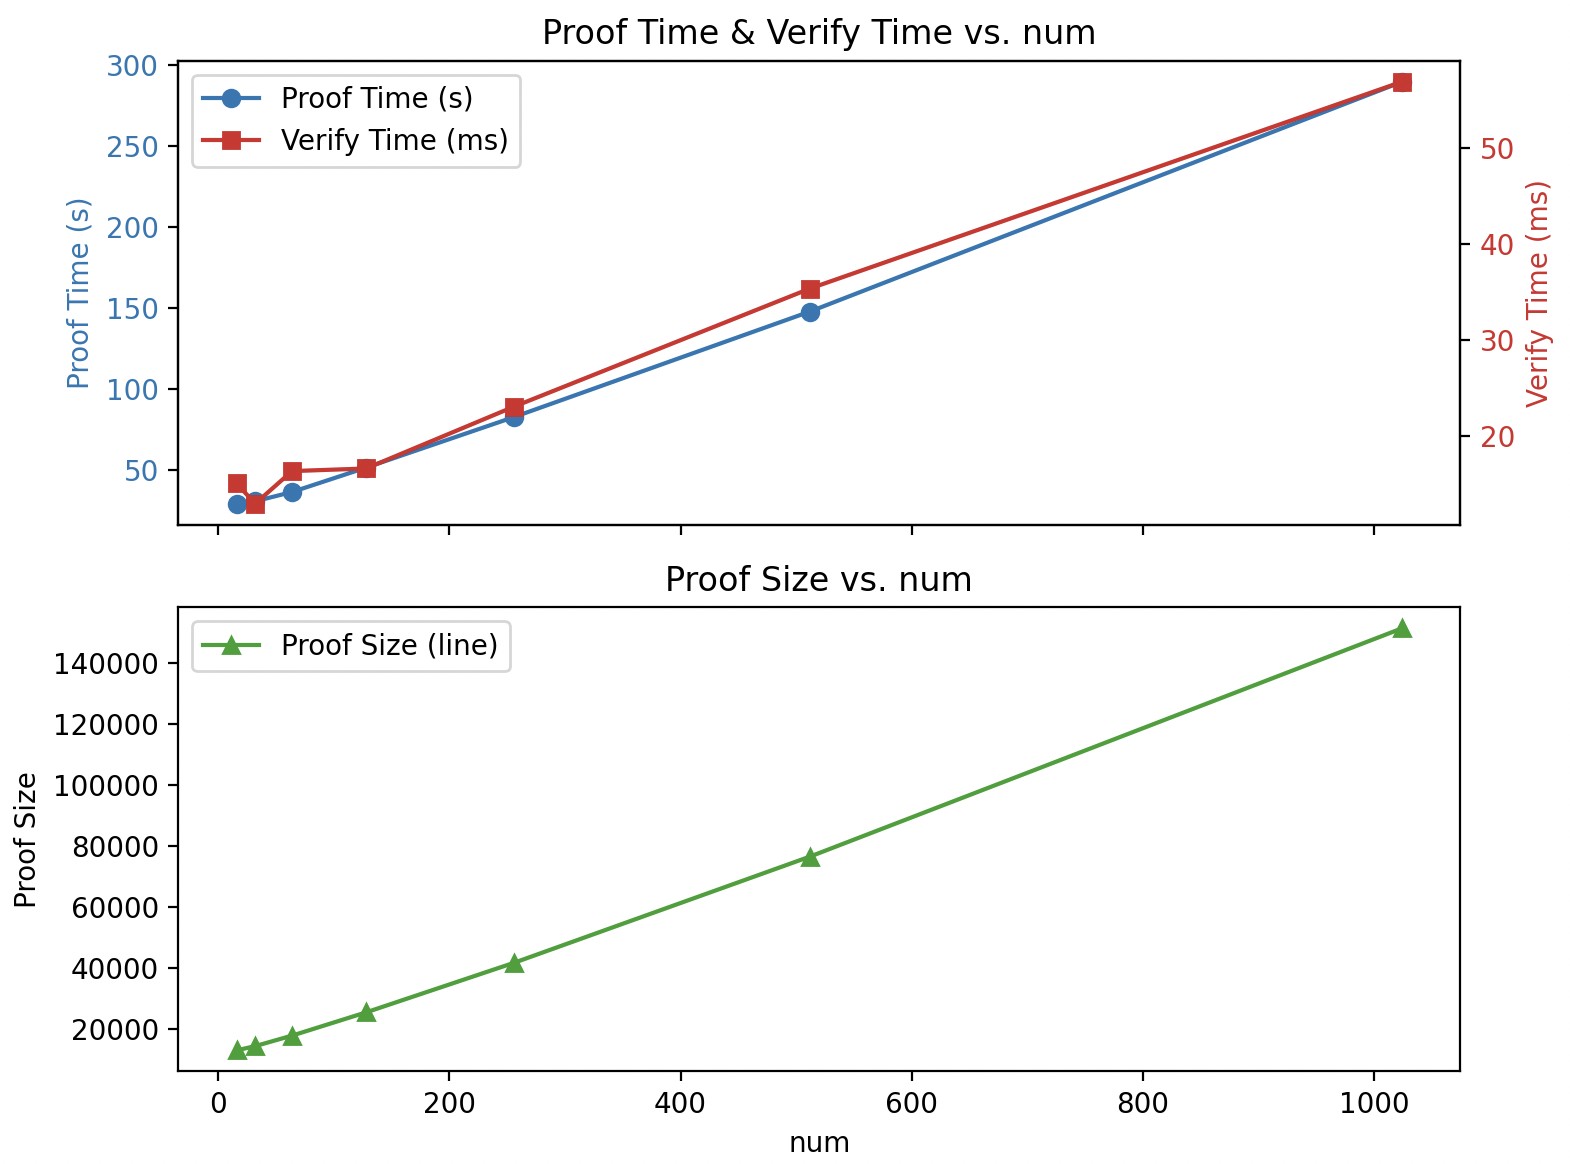
\includegraphics[width=1\linewidth]{test2.png}
    % \caption{Enter Caption}
    \label{fig:enter-label}
\end{figure}



\subsection{Performance Comparison}

As we discussed above, when turns to BLS signature scheme, the original proving method(relations in the paper) will be very costly. So we choose to prove the aggregation key and verify the ATMS signature.

Below is our benchmark result of our proposal:


\begin{table}[H]
\centering
\begin{tabular}{c|c|c|c}
\hline
\textbf{num} & \textbf{proof\_time} & \textbf{proof\_size} & \textbf{verify\_time} \\ \hline
3 of 6 & 25.27s & 11872 & 13.42ms \\
6 of 9 & 26.81s & 12224 & 12.45ms \\
8 of 9 & 26.59s & 12224 & 12.07ms \\
14 of 21 & 27.51s & 12576 & 14.54ms \\
17 of 21 & 27.45s & 12576 & 13.15ms \\
28 of 42 & 28.80s & 13376 & 11.48ms \\
72 of 102 & 32.13s & 15104 & 13.80ms \\
1602 of 2001 & 160.75s & 80192 & 39.05ms \\ \hline
\end{tabular}
\caption{Proof Time, Proof Size and Verify Time for ATMS in BLS}
\end{table}


And we made a quick comparison of two ATMS proving method, only compare the proving time:




\begin{table}[htbp]
\centering
\begin{tabular}{c|c|c}
\hline
\textbf{num} & \textbf{BLS ATMS} & \textbf{Schnorr ATMS}  \\ \hline
3 of 6 & 25.27s & 1.72s  \\
6 of 9 & 26.81s & 2.90s  \\
8 of 9 & 26.59s & 2.93s \\
14 of 21 & 27.51s & 4.73s  \\
17 of 21 & 27.45s & 8.01s  \\
28 of 42 & 28.80s &8.36s  \\
72 of 102 & 32.13s & 30.52s  \\
1602 of 2001 & 160.75s &  292.39s \\ \hline
\end{tabular}
\caption{ATMS Proving Time Comparison}
\end{table}


The reason why BLS ATMS's proving time do not show significant changes in aggregation number is that we did not customize circuit's degree, but it is actually a $O(n)$ algorithm. 

Note that these two versions of ATMS benchmarks are running over very different settings, following is the information:

\begin{table}[htbp]
\centering
\begin{tabular}{c|c|c}
\hline
\textbf{} & \textbf{BLS ATMS} & \textbf{Schnorr ATMS}  \\ \hline

machine & Linux Server & Linux Server \\ \hline
library & halo2-lib & sidechains-zk \\ \hline
curve & bn254& bls12-381/jubjub \\ \hline
hash& Poseidon& Rescue \\ \hline

\end{tabular}
\caption{ATMS Benchmark Settings}
\end{table}


The CPU of our linux server is Intel Xeon Silver 4214 (48 cores)@3.2GHz, and the RAM is 128GB.

Although the Schnorr ATMS(original SNARK-based ATMS) is working on the bls12-381 curve, it use a embedding curve named jubjub, whose base field is the scalar field of bls12-381, with a length of 255-bit. And we benchmark our BLS ATMS over curve BN254, so according to the benchmark settings, our BLS ATMS is more efficient in proving time.



\section{ATMS VS Mithril}


\subsection{Application and Use Case}

\textbf{ATMS},
from the \textit{Proof-of-Stake Sidechains} paper, is a signature scheme designed for sidechains' certificate:

\vspace{0.3cm}

\textit{An important feature of our construction is merged-staking
that prevents "goldfinger" attacks against a sidechain that is only carrying a small amount of stake. An important technique for pegging chains that we use in our construction is cross-chain certification which is facilitated by a novel cryptographic primitive we introduce called ad-hoc threshold multisignatures (ATMS) which may be of independent interest. We show how ATMS can be securely instantiated by regular and aggregate digital signatures as well as succinct arguments of knowledge such as STARKs and bulletproofs with varying degrees of storage efficiency}

\vspace{0.3cm}

The nodes on the mainchain will get information from sidechains, and the information allow them to authenticate a small number of stakeholders on the sidechains, whom are trusted to present a majority of all stakeholders. The information changes periodly, since the stake distribution is a dynamic value.


All the transactions and authentication information will be packed per "epoch", the paper call it a \textit{cross-chain certification}.


\vspace{0.3cm}


\textbf{Mithril}, from the paper \textit{Mithril: Stake-based Threshold Multisignatures}, is a signature scheme designed for mainchain's certificate:

\vspace{0.3cm}

\textit{We also examine the problem of bootstrapping light clients in Proof of Stake
(PoS) blockchains. The general challenge in this setting is that the client needs
to verify the ledger upon joining the network and that block verification fundamentally depends on stake (unlike an SPV client in the bitcoin setting, that can
simply count the blocks’ aggregate difficulty). As a result, a client bootstrapping
in the PoS setting needs to follow the stake as it moves between accounts to be
in sync over time with the stakeholder distribution and validate all the blocks.
The amount of work to be performed scales linearly with the number of transactions in the ledger which can be extremely large. Using mithril, a different
approach can be followed: instead of verifying transactions, the stakeholders can
issue checkpoints at regular intervals using an STM signature. The client needs
only to verify all checkpoints till the most recent one after which individual
blocks and transactions can be verified sequentially. In this way the operation
becomes linear in the number of checkpoints instead of linear in the number
of transactions. The frequency of the checkpoints can be set to be at regular
intervals.}

\vspace{0.3cm}

In our zero-knowledge bridge context, we refer to the second application in the Mithril paper, that is the quick bootstrapping of Mithril light client(Cardano light client). The Mithril protocol provides Blockchain checkpoints periodly, and the light client can verify the Mithril certificates continuously.

\vspace{0.3cm}

We offer a quick comparison of two schemes:

\begin{table}[htbp]
    \centering
    \renewcommand{\arraystretch}{1.1} % 增加行间距
    \setlength{\tabcolsep}{10pt}      % 增加列间距
    \begin{tabular}{c|c|c} \hline
         & \textbf{Mithril} & \textbf{ATMS}   \\ \hline
        core signature  & BLS  & Schnorr/BLS    \\
        aggregation & complex & simple \\
        proving task& heavy & light \\
        target& N/A &mainchain \\
        participation & low percentage & high percentage \\ 
        use case& bootstrapping & cross-chain \\ \hline
    \end{tabular}
    \label{tab:example_benchmark_selected}
\end{table}

The ATMS is used for blockchain's interoperability, but as described in the paper, ATMS signature can only be verified on the mainchain. So if we want to construct a bridge using ATMS, it can only bridge from a sidechain to Cardano mainchain.

While Mithril is not designed for cross-chain, and the "light client" use case of Mithril allow it to be used for bridge. Thus if we construct a bridge using Mithril, it can bridge from Cardano to "any" other blockchain(whether in the same ecosystem or not).

\subsection{Proving the Certificate}

Both two multisignature schemes, Mithril and ATMS, can be used to "sign" the certificate. Although two certificates have a significant difference, the ZK system do the same thing -- proving the correctness of multisignature. 

There is a subtle but not very important issue, that is the relations(need to prove) in the Mithril paper do not include the signature verification, which means that the verifier need to validate the multisignature itself. While in the SNARK-based ATMS(both Inigo's implementation and our proposal), the ZK-SNARK just prove the multisignature verification in the circuit, thus the verifier only verify the ZK proof. For convenience, we agreed to prove the signature in SNARK-based Mithril, although it is inconsistent with paper.


As we mentioned above, two multisignature schemes have different use cases, so the relations need to prove are also dissimilar. In our understanding, we need to prove the eligibility of signers in SNARK-based Mithril. But in SNARK-based ATMS, this step is not necessary, because all qualified signers were committed(as a product) in the "genesis" block.

Here we give a rough introduction of relations in two multisignature schemes.

\vspace{0.3cm}
\textbf{SNARK-based Mithril}(see specific relations in Section 5.1, Mithril paper):

\begin{itemize}
    \item \textbf{Signature Check}: including the correctness of verification keys($avk$) and multisignature($\sigma$), as well as multisignature verification(if needed).
    \item \textbf{Consistence Check}: including the Merkle tree memebership check, and the lottery index check(each signer must hold a unique lottery index).
    \item \textbf{Eligibility Check}: including the mapping function(we use hash function to replace Elligator Squared) and the comparison between $ev$ and signer's stake.
\end{itemize}

\vspace{0.3cm}


\textbf{SNARK-based ATMS}(see specific relations in Section 5.3 ATMS paper and this report):

\begin{itemize}
    \item \textbf{Inigo's implementation}: check that all keys are hashed to a specific value, and check signatures one by one. The number of valid signatures achieves the threshold.
    \item \textbf{Our proposal}: check every key used to aggregate the $avk$ is a member of pre-committed Merkle tree, and the multisignature is computed by the corresponding keys. Also the aggregated verification key $avk$ can correctly verify the multisignature.
\end{itemize}

\subsection{Implementation Details}


Similarly to the SNARK-based ATMS with BLS signature, we implemented SNARK-based Mithril in the open source library "halo2-lib". And the SNARK-based ATMS with Schnorr signature is in crate "sidechains-zk". These two crates have significant deiiferences, below, we list some of their settings and details:

\begin{table}[H]
    \centering
    \begin{tabular}{c|c|c} \hline
        & sidechains-zk & halo2-lib \\ \hline
       Curve&  bls12-381/jubjub& bn254, secp256k1, grumpkin  \\ 
       Hash Function& Rescue &Poseidon, SHA256, Keccak \\ 
       Hash Rate & 3 & adjustable \\ 
       Signature scheme& Schnorr, EdDSA& BLS, Schnorr, EcDSA \\ 
        Gate Region& Fixed & Flexible \\ \hline
    \end{tabular}
    \caption{Comparison of libraries}
    \label{tab:my_label}
\end{table}


Next, we will provide necessary explanations for some fields in the above table:

\begin{itemize}
    \item \textbf{Curve}: "sidechains-zk" use bls12-381 and its embedding curve, jubjub. The official implementation of "halo2-lib" only have three curves, but the community has various implementation of other curves, like bls12-381 and secp256k1.
    
    \item \textbf{Hash Function}: "sidechains-zk" implemented Rescue, with a fixed hash rate equals to 3. While "halo2-lib" has three hash function, including one SNARK-friendly hash Poseidon and two used in Ethereum, SHA256 and Keccak. Especially, we can adjust the hash rate of Poseidon hash function, which bring convenience to our implementation.

    \item \textbf{Signature Scheme}: "halo2-lib" implemented the pairing circuit, thus made BLS signature proving practical. And "halo2-lib" also have the mechanism like field extension, which means that we can operate $\mathbb
    {G}_2$ or $\mathbb{G}_{12}$ group element in the circuit.

    \item \textbf{Gate Region}: "sidechains-zk" has a fixed gate configuration, it likes a Plonkish arithmetization, every row has 5 advice columns, and some fixed columns. The gate configuration in "halo2-lib" can be adjust dynamically, we can change the number of rows, total columns will also change accordingly.
    
\end{itemize}



\end{document}
